\documentclass[10pt]{article}
\usepackage{icmlko}

\icmlmeta{IP 파운데이션 월드모델}{53}{자유도가 아니라 대응이었다}{한 노트 만에 스스로 반증한다 --- 잡음 축은 끄는 것보다 나쁘고, 값이 아니라 어느 레코드의 값인지가 전부다}

\begin{document}

\twocolumn[
\icmlheader

\begin{abstract}
노트 52는 매장 노출도 축의 가치가 ``라벨 설명력이 아니라 정렬 자유도''라고
했다 --- 내용을 세 배 좋게 해도 $+$0.002인데 없애면 $-$0.031이므로, 공통 축이
셋이냐 둘이냐가 축 내용보다 크다고 본 것이다. 같은 노트에 반증 조건을 적었다:
``자유도가 이유라면 아무 값이나 넣어도 축을 켜는 것만으로 회복돼야 한다.''
검정했다. \textbf{반증됐다.} 잡음 축은 회복하지 못할 뿐 아니라 \emph{끄는 것보다
나쁘다}($+$0.3002 대 $+$0.3135, 회복률 $-$43\%). 여섯 도메인 전부에 잡음 축을
켜면 $+$0.1935까지 떨어진다. 판별 검정을 하나 더 했다 --- 실제 축 값을 그대로
두고 \emph{어느 레코드의 값인지만} 섞었다. 분포는 완전히 같고 대응만 깨진다.
$-$0.0352로 끄는 것($-$0.0312)과 같아진다. \textbf{축의 가치는 값의 분포도
축의 존재도 아니고 레코드 수준의 대응이다.} 그러면 노트 52의 진짜 질문 ---
왜 내용을 개선해도 안 오르나 --- 은 다르게 답해야 한다. 현행 축과 `최대 규모'의
상관을 재니 도서 $+$0.836, 웹툰 $+$0.655, 게임 $+$0.646으로 \textbf{현행 축이
이미 42--70\%를 담고 있다.} 개선의 여지가 없어서 안 오른 것이다. 도메인별
기여는 신호 강도와 표본 크기의 곱을 따른다 --- 웹툰(n$=$900, r$=+$0.087)이
$-$0.0433으로 가장 크고 도서(n$=$243, r$=+$0.030)는 $+$0.0014로 있으나 마나다.
\end{abstract}
]

\section{반증 조건을 바로 검정했다}

노트 52의 주장은 이랬다.

\begin{quote}\fontsize{9.5}{11.5}\selectfont
``공통 축의 가치는 두 종류다 --- 라벨을 설명하는 몫과 정렬에 쓰이는 몫.
매장 노출도는 앞의 것이 약하고 뒤의 것으로 값을 한다.''
\end{quote}

그리고 반증 조건을 함께 적었다 --- ``자유도가 이유라면 아무 값이나 넣어도
축을 켜는 것만으로 회복돼야 한다.''

\begin{figure}[t]
\centering
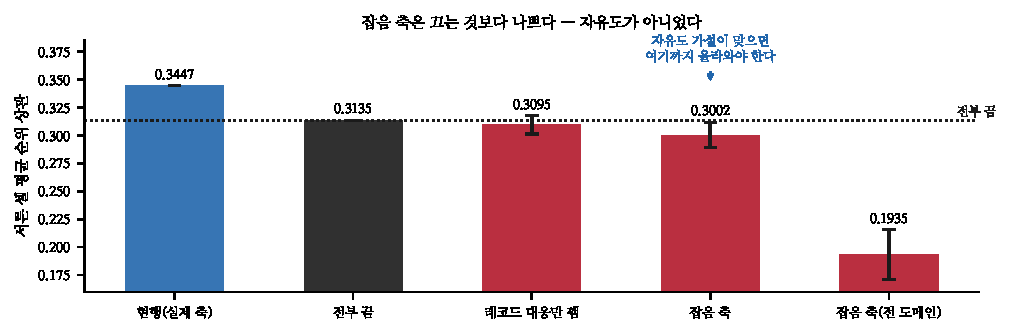
\includegraphics[width=\textwidth]{figs/falsify.pdf}
\caption{네 조건. 오차 막대는 씨앗 여덟 개의 표준편차다.}
\end{figure}

\begin{table}[t]
\centering\tsize
\caption{매장 노출도 축을 바꿔 가며.}
\begin{tabular}{lr}
\toprule
조건 & 서른 셀 평균 $\rho$ \\
\midrule
현행(실제 축) & $+$0.3447 \\
전부 끔 & $+$0.3135 \\
레코드 대응만 깸 & $+$0.3095 \\
\textbf{잡음 축}(마스크 유지) & \textbf{$+$0.3002} \\
잡음 축(여섯 도메인 전부) & $+$0.1935 \\
\bottomrule
\end{tabular}
\end{table}

\textbf{잡음 축은 끄는 것보다 나쁘다.} 자유도 가설이 맞으면 $+$0.3447 근처까지
올라와야 하는데 $+$0.3002로 내려간다. 회복률이 $-$43\%다.

\claimx{노트 52의 ``정렬 자유도'' 설명을 철회한다. 공통 축을 하나 더 갖는 것
자체는 값을 하지 않으며, 잡음으로 채우면 거짓 대응이 생겨 오히려 해롭다.}
{잡음의 분포가 실제 축과 달라서일 수 있으므로 다음 검정이 필요했다.}

\section{분포는 같고 대응만 깨면}

잡음은 값의 분포도 다르다. 그래서 실제 축 값을 그대로 두고 \emph{어느 레코드의
값인지만} 섞었다. 분포는 완전히 같고 레코드 대응만 깨진다.

\begin{table}[t]
\centering\tsize
\caption{대응을 깰 때.}
\begin{tabular}{lrr}
\toprule
& $\rho$ & 현행 대비 \\
\midrule
현행 & $+$0.3447 & --- \\
전부 끔 & $+$0.3135 & $-$0.0312 \\
\textbf{레코드 대응만 깸} & $+$0.3095 & \textbf{$-$0.0352} \\
\bottomrule
\end{tabular}
\end{table}

대응을 깨면 끄는 것과 같아진다.

\claimx{매장 노출도 축의 가치는 값의 분포도 축의 존재도 아니고 \textbf{레코드
수준의 대응}이다 --- 이 레코드의 이 값이 맞아야 한다.}{도메인 간 대응(같은 물리량)과
레코드 내 대응을 여기서 구분하지 않았다. 도메인 간에만 섞는 검정이 남아 있다.}

노트 20·23에서 ``같은 물리량이어야 한다''는 정합 제약을 원칙으로 두었는데,
그것이 여기서 정량적으로 확인된다. 축이 있다는 사실이 아니라 축이 각 레코드에
대해 옳다는 사실이 전이를 만든다.

\section{그럼 왜 개선이 안 옮겨졌나}

노트 52가 던진 질문은 남는다 --- 사전 이력을 최대 규모로 바꿔 단독 상관을 세
배로 키웠는데 왜 전체가 $+$0.002뿐인가.

\begin{figure}[t]
\centering
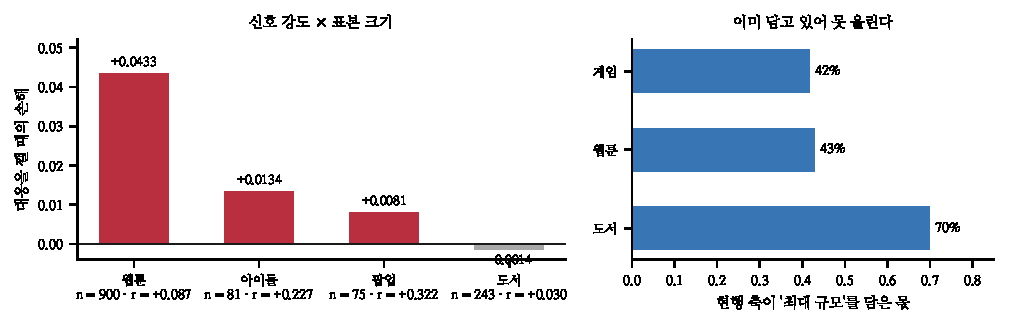
\includegraphics[width=\textwidth]{figs/contrib.pdf}
\caption{왼쪽 --- 도메인별 기여. 오른쪽 --- 현행 축이 이미 담은 몫.}
\end{figure}

\begin{table}[t]
\centering\tsize
\caption{현행 매장 노출도 축과 `최대 규모'의 관계.}
\begin{tabular}{lrr}
\toprule
도메인 & 상관 & 설명된 몫 \\
\midrule
도서 & $+$0.836 & 70\% \\
웹툰 & $+$0.655 & 43\% \\
게임 & $+$0.646 & 42\% \\
\bottomrule
\end{tabular}
\end{table}

\textbf{현행 축이 이미 42--70\%를 담고 있다.} 건수와 최대 규모가 서로 상관되므로
바꿔도 새 정보가 절반 이하만 들어온다. 개선의 여지가 없어서 안 오른 것이지
축이 무의미해서가 아니다.

\section{어느 도메인이 이 축을 필요로 하나}

\begin{table}[t]
\centering\tsize
\caption{도메인별로 대응을 깰 때의 손해.}
\begin{tabular}{lrrr}
\toprule
도메인 & n & 축 신호 r & 손해 \\
\midrule
\textbf{웹툰} & 900 & $+$0.087 & \textbf{$-$0.0433} \\
아이돌 & 81 & $+$0.227 & $-$0.0134 \\
팝업 & 75 & $+$0.322 & $-$0.0081 \\
도서 & 243 & $+$0.030 & $+$0.0014 \\
\bottomrule
\end{tabular}
\end{table}

기여가 신호 강도와 표본 크기의 곱을 따른다. 웹툰은 축 신호가 $+$0.087로 약한데
n$=$900이라 가장 크게 기여하고, 도서는 n$=$243인데 신호가 $+$0.030으로 약해
있으나 마나다. \textbf{팝업은 축 신호가 가장 강한데($+$0.322) n$=$75라 손해가
$-$0.0081에 그친다} --- 표본이 병목이라는 것이 여기서도 확인된다.

\section{한계}

\begin{itemize}[leftmargin=1.1em,itemsep=0.15em]
\item 도메인 간 대응과 레코드 내 대응을 구분하지 않았다. 한 도메인의 축을 다른
      도메인으로 옮겨 보는 검정이 남아 있다.
\item 잡음을 균등분포로 만들었다. 실제 축의 분포를 흉내 낸 잡음이면 결과가
      덜 극단적일 수 있다(대응 깨기가 그 역할을 했지만 완전히 같지는 않다).
\item 도메인별 손해를 각각 다섯 씨앗으로만 쟀다.
\item ``신호 강도 $\times$ 표본 크기''는 네 점에서 눈으로 본 것이고 회귀하지
      않았다.
\item 노트 52를 철회하지만 그 노트가 던진 질문(왜 개선이 안 옮겨지나)의 답은
      바뀌었을 뿐 질문 자체는 옳았다.
\end{itemize}

\section{다음}

\begin{enumerate}[leftmargin=1.3em,itemsep=0.15em]
\item 도메인 간 축 교환 --- 대응의 층위를 가른다.
\item 웹툰 매장 노출도를 강화한다. 신호가 $+$0.087로 약한데 기여가 가장 크므로
      개선 여지가 가장 크다.
\item 도서 매장 노출도는 사실상 무용하다. 다른 물리량으로 바꿀 후보를 찾는다.
\item 팝업 표본 --- 축은 가장 좋은데 표본이 병목이라는 것이 또 확인됐다.
\end{enumerate}

\vspace{0.6em}
\hrule height 0.3pt
\vspace{0.5em}
{\footnotesize
\textbf{참고문헌}\\[0.3em]
Meredith, W. (1993). Measurement invariance, factor analysis and factorial
invariance. \emph{Psychometrika}, 58(4), 525--543.\\[0.15em]
Schönemann, P. H. (1966). A generalized solution of the orthogonal Procrustes
problem. \emph{Psychometrika}, 31(1), 1--10.\\[0.15em]
Good, P. (2005). \emph{Permutation, Parametric, and Bootstrap Tests of
Hypotheses}, 3rd ed. Springer.\\[0.15em]
Gower, J. C., Dijksterhuis, G. B. (2004). \emph{Procrustes Problems}.
Oxford University Press.\\[0.15em]
Ben-David, S. et al. (2010). A theory of learning from different domains.
\emph{Machine Learning}, 79(1--2), 151--175.
}

\end{document}
